
%%% Local Variables: 
%%% mode: latex
%%% TeX-master: t
%%% End: 

\chapter{需求分析与系统框架设计}

\section{业务需求分析}

如今,走向科学化、信息化,通过数据来分析才能更好的进行诊疗,当代医学的已经不能再仅仅依靠医生的经验通过望闻问切进行诊断。如之前所阐述,认知功能障碍表现多样而导致诊断需要针对患者的各项能力进行评测,并通过均衡各项的分数而得出结论。由于传统纸笔测试的繁琐、学习成本大、题量繁多,导致数据不易存储、诊断不方便、学习代价大等等困难。而开发这样一款电子问卷可以很好的解决这些问题,能够更好地组织所有的数据。同时,波士顿大学和北京协和医院都和我们提出了合作的请求,希望开发这样的方便的系统辅助医生进行诊断和数据整理。开发这样的脑健康评估系统是走在了中国乃至世界脑健康研究的前列,可以推动脑健康研究的发展,也可以巩固合作医院的业界地位。

\section{功能需求分析}

脑健康研究系统要求完成一个辅助医生诊断认知功能障碍的系统。系统包括多种题目包括信息录入、选择题、录音题、画图题。最终系统需要对用户录入的信息进行统计整理、并对做的题目进行评分(画图题只需针对流畅性给出辅助性的评分,语音题能够做一些适当的识别,其余需要根据评分标准给分),对认知功能障碍做一个初步的诊断。

\subsection{故事复述题}

\begin{figure}[h]
  \centering
  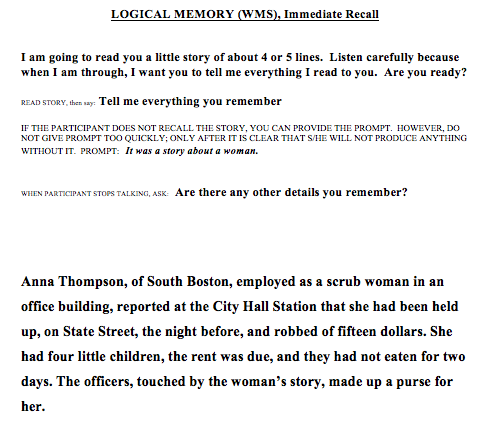
\includegraphics[width=13cm]{chapter2-1}
  \caption{原问卷中的故事复述题}
\end{figure}

故事复述题为医生为病人讲述一个4-5行的小故事,然后让病人立即复述这个故事的内容,医生可以给一些提示(如“这是一个关于女人的故事”)。变为电子问卷后需要拥有以下需求:

\begin{itemize}
\item 存储故事的录音、可以播放故事的录音。
\item	可以将病人全部的讲述的音频录制下来并保存、后期可以调出录音进行评分。
\item 与问卷一样拥有提示语句。
\end{itemize}

另外希望能够为该类型的题目提供辅助打分功能:

\begin{itemize}
\item 播放测试时录制的病人陈述。
\item	对录音进行语音识别。
\item	与打分问卷一样的打分版面。
\end{itemize}

\subsection{图片复原题}

\begin{figure}[h]
  \centering
  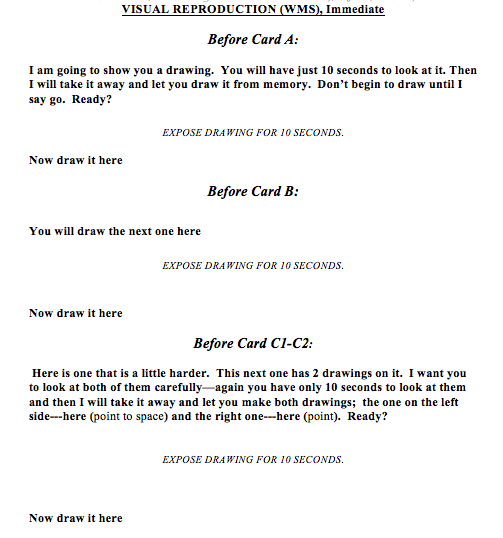
\includegraphics[width=13cm]{chapter2-2}
  \caption{原问卷中的图片复原题}
\end{figure}

图片复原题为医生会给病人依次展示三张图片卡片(每个展示十秒),结束后记录病人绘画的轨迹。变为电子问卷后需要拥有以下需求:

\begin{itemize}
\item 可以存储需要展示的图片、并能控制其显示十秒钟后消失。在图片展示时,提示语句不应该出现。
\item	能记录病人绘画的轨迹过程。在绘画后面的图片时,前面的图片应该还在其视野中。
\item 与问卷一样拥有提示语句。
\end{itemize}

另外希望能够为该类型的题目提供辅助打分功能:

\begin{itemize}
\item 展示病人之前绘画的轨迹。
\item	与打分问卷一样的打分版面。
\end{itemize}

\subsection{单词配对题}

\begin{figure}[h]
  \centering
  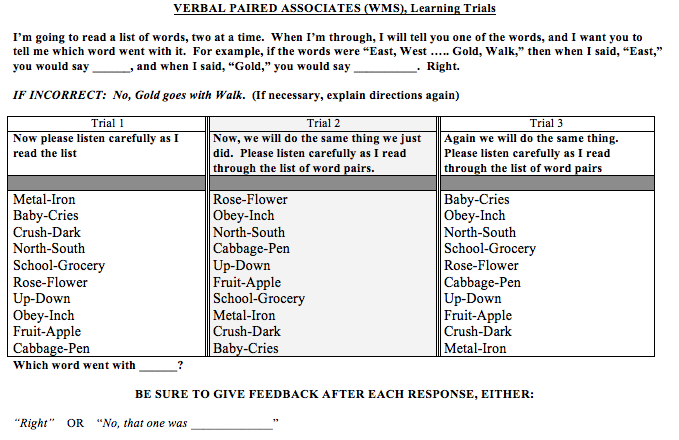
\includegraphics[width=13cm]{chapter2-3}
  \caption{原问卷中的单词配对题}
\end{figure}

单词配对题为医生会为病人读连续十个单词对,之后向病人进行提问,根据病人回答的单词进行评分(分为正确、有关错误、无关错误、搞混错误)。变为电子问卷后需要拥有以下需求:

\begin{itemize}
\item 可以存储读单词对的录音并进行播放。
\item	界面能便于医生进行答案记录和打分。
\item	需要记录错误答案的类型(以字典形式)。
\item	能够根据选择计算总得分。
\end{itemize}

\subsection{延期复述题}

\begin{figure}[h]
  \centering
  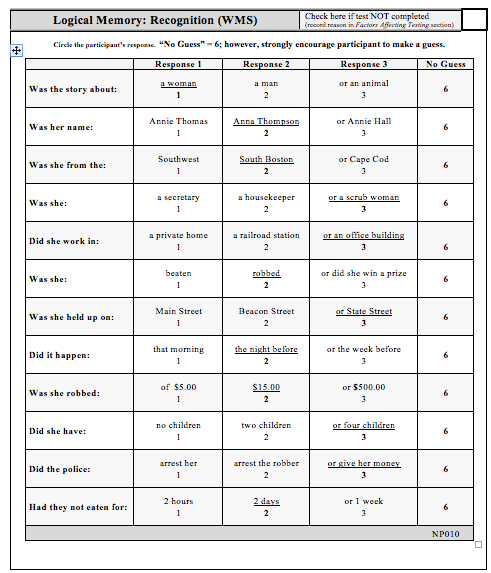
\includegraphics[width=13cm]{chapter2-5}
  \caption{原问卷中有关故事复述的延期复述题}
\end{figure}

很多类型的题目都拥有延期复述题(如故事复述题、图片复原题、单词配对题都有),是在这些题目测试结束之后一段时间再进行测试,主要考察病人的长期记忆力。该题目主要是选择题(但也有其他题目类型)。变为电子问卷后需要拥有以下需求:

\begin{itemize}
\item 可以展现题目、并能让医生方便的看出正确答案。
\item	能够方便的记录病人的回答,也能对病人的答案进行“一键式”评分。
\end{itemize}

\subsection{数字串复述题}

\begin{figure}[h]
  \centering
  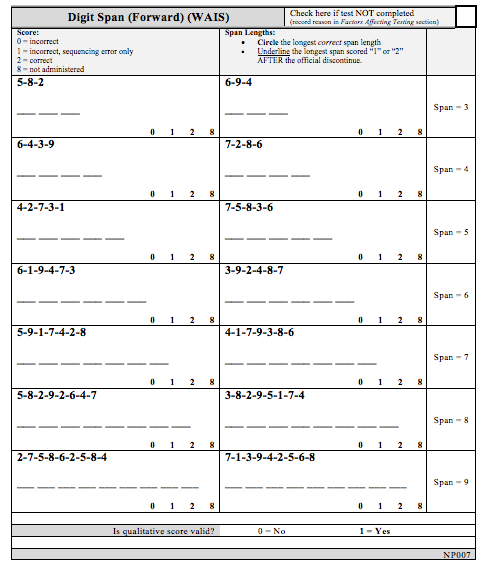
\includegraphics[width=13cm]{chapter2-4}
  \caption{原问卷中的数字串复述题}
\end{figure}

数字串复述题分为两类,一类为“顺序”,另一类为“逆序”。顺序数字串复述题为医生为病人说一串数字,病人需要按照顺序复述;逆序数字串复述题则需要病人按照逆序复述,逆序数字串复述题还拥有引导病人的两道题目。如果病人数字和顺序都正确,则可以获得两分,如果只有数字是正确的,则可以获得1分,否则只有0分。该题目最终得分为两个数值,一个是最长正确复述数字串长度,另一个是无关顺序最长正确复述数字串长度,每个长度的数字串有两道题目,如果都得了0分则测试结束。变为电子问卷后需要拥有以下需求:

\begin{itemize}
\item 展现题目、能够方便记录病人答案,也能让医生方便的看到正确答案。
\item	能够计算两个分值:最长正确复述数字串长度和无关顺序最长正确复述数字串长度。
\item 能够对医生做一定引导,告诉医生下一个测试的数字串是什么。
\end{itemize}

\subsection{其他需求分析}

其他需求包括界面的要求、网络的要求等等,主要归纳如下。

\begin{itemize}
\item 需要与纸板问卷有一样的体验,展示界面应该和标准A4纸大小类似。
\item	界面应该尽量还原原来问卷的界面,并且对使用者有一定引导性、方便好用。
\item 能有效组织题目和病人数据。
\item 界面友好。
\end{itemize}

\section{系统框架设计}

\begin{figure}[h]
  \centering
  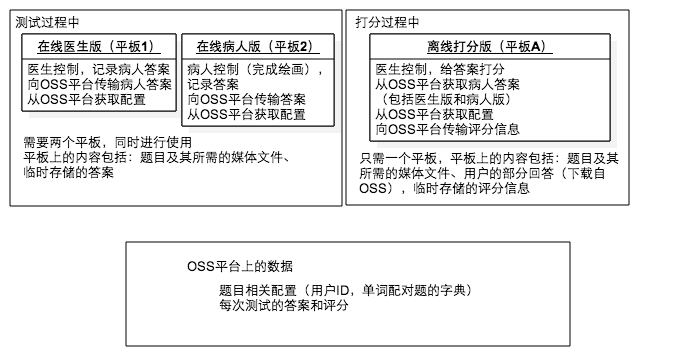
\includegraphics[width=13cm]{struct}
  \caption{三个版本的关系说明图示}
\end{figure}

根据上述需求,最终设计的系统分成三个版本:在线医生版、在线病人版和离线打分版,并用JSON格式化了整个系统的数据(包括题目的存储和病人的回答),以及用Java面向对象的继承特性设计大体框架和底层逻辑。

\subsection{三个版本}

为了满足和纸板问卷一样的体验的要求,并且保证开发过程中的便捷,整个系统分成三个独立的版本,两个在线版本用来复原原问卷的测试部分,而离线版本可以对测试得到的结果进行一定的评分和修正。这三个版本虽然没有相互的通讯,但是共享一个数据库(题目和测试结果),保持了开发的简单性和数据的统一性。

\subsubsection{在线医生版}

在线医生版为医生在测试时使用的,涵盖了原问卷大部分的题目(如故事复述题)。该版本不仅需要还原原问卷上的这些题目,也需要给医生提供一些引导语句和引导图示,同时也需要针对操作失误进行防范。

\subsubsection{在线病人版}

在线病人版为病人在测试时使用的,主要为了满足原问卷中一些医生和病人都需要纸板问卷的题目(如图片复原题)。不合并在线医生版和病人版的原因是这样不仅可以和原问卷这些题目一样双方都拥有问卷的体验,同样也将一些题目拆分开,使开发过程中一类题目不用分成两种不同的实现版本,更加简化了设计和开发。

\subsubsection{离线打分版}

离线打分版用于在测试过后医生重新调出之前测试的结果并进行打分,在这个版本中不仅需要给出人工评分、勾选的功能,也需要设计一些自动算法进行辅助性评分(如进行语音识别、轨迹识别等)。

\begin{figure}[h]
  \centering
  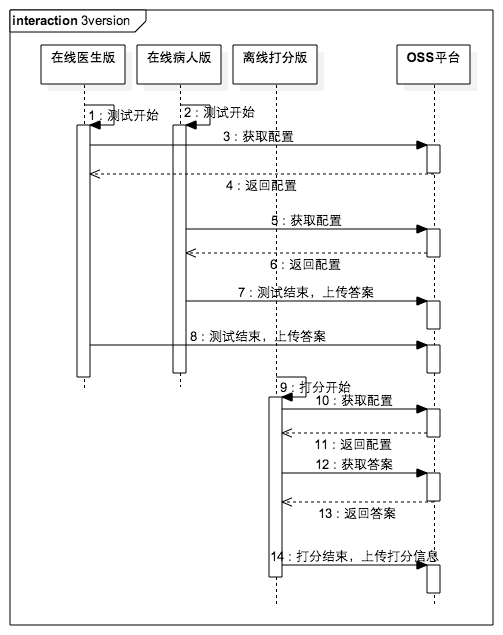
\includegraphics[width=13cm]{3version}
  \caption{一次测试中三个版本的使用说明图}
\end{figure}

\subsubsection{三个版本的关系说明}

在测试时,分别使用两个平板作为使用在线医生版和在线病人版的媒介并分别给予病人和医生使用。平板上存储有关题目的所有信息(包括媒体文件),但是需要从OSS平台上下载配置(因为题目的不变性和配置需要改变的特性)。在测试结束后要向OSS平台上传该测试得到的答案。

在打分时,只需要一个平板(可以复用在测试时使用的在线医生版)用于医生使用。平板上存储有关题目的所有信息,同在线版本一样需要从OSS平台上下载配置,也需要在OSS平台上下载用户的相关答案。在打分结束后需要向OSS平台上传打分的信息。

\subsection{数据系统设计}

在这次系统设计中,题目有关的数据存在了APP内部(Android工程的res文件下),包括题目的文字、画图题的图片、音频题需要播放的录音,这样保证在APP上题目可以瞬间读出而不需要再从网络上获取,因为题目已经固定无需修改,固定在APP中使得这些数据不会遭到操作失误而导致的修改,也使得逻辑部分的实现变得简单。而病人的测试数据和结果、以及APP的一些配置文件放在阿里云的开放存储平台上,这样可以使三个版本都能方便的读取、修改和评分。其中题目的文字和病人的一些可以用文字表达的答案均使用了JSON格式化。

这样的数据系统具有性能快、开放、安全、可靠、可操作性强等特点。

\subsubsection{JSON格式介绍}

JSON(全程JaveScript Object Notation)是一个轻量级的数据交换语言,以文字为基础,且易于让人阅读,现在已经成为一个独立于语言的文本格式。JSON用于描述数据结构,有以下形式存在:

\begin{itemize}
\item 对象:一个对象以左花括号开始,用右花括号结束。一个对象包含一些列并序列的名称-值对,每个名称-值对之间使用逗号分割。
\item 名称-值:名称和值之间使用冒号分割,一般形式为:
\begin{lstlisting}[language=JAVA]
{name:value}
\end{lstlisting}
其中名称一定是一个字符串(用双引号扩起来的一串字符),一个值可以是一个字符串,可以是一个数值(一系列0-9的数组组合,也可以是负数或小数,也支持用e或E表示指数形式),可以是一个布尔值(true或false),可以是一个对象,可以是一个有序列表,也可以是一个空值(null)。
\item 值的有序列表:一个或者多个值用逗号分区后,使用左大括号和右大括号括起来的一个列表,如:
\begin{lstlisting}[language=JAVA]
[collection, collection]
\end{lstlisting}
\end{itemize}

JSON由于其便捷、易懂、表达能力强的特性应用范围广泛。在数据系统的设计中使用JSON是因为可以方便的利用它定义任何文字表达的数据,且在Java的内部库中已经包含了对JSON格式读取、存储的API,使利用JSON开发数据系统的代价非常小。

\subsubsection{题目资源数据}

这部分由于数据的固定性,也为了开发的方便,直接固定在了APP内部,均存放在Android工程的res文件下。其中题目用JSON格式化,这样便于不同题目类型可以统一地存放在一个文件中,也方便后续对新题型进行扩展,同时也容易修改或者增加其他新的特征(原题目和JSON格式化后的示例可以见图3.8)。

\begin{figure}[h]
\centering%
\begin{subfigure}{13cm}
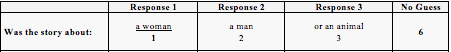
\includegraphics[width=13cm]{JSON_OQ}
\caption{原问卷中的题目}
\end{subfigure}
%\hspace{4em}%
\begin{subfigure}{6cm}
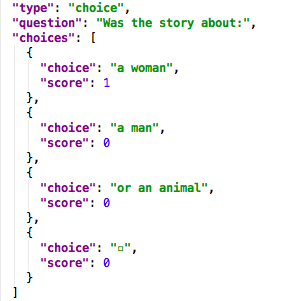
\includegraphics[width=6cm]{JSON_Q}
\caption{JSON格式化的题目}
\end{subfigure}
\hspace{4em}%
\begin{subfigure}{6cm}

\includegraphics[width=6cm]{JSON_A}
\caption{JSON格式化的示例答案}
\end{subfigure}
\caption{题目和对应题目JSON、答案JSON示例}
\label{fig:big1-subfigure}
\end{figure}

JSON格式化后的题目主要包含以下几个名称-值对:

\begin{itemize}
\item type(类型):表示当前题目的类型,有choice(选择题)、story\_recall(故事复述题)、digit\_span(数字串复述题)、trailer(单词配对题)、draw(图片复原题)等。
\item guide\_word(引导词):表示该题目的引导词。
\item record(记录名):说明该题目需要进行音频录制,此值表示的是需要上传录音文件的名字。
\item skip(跳过):表示如果该题目被跳过,则这个值中的题目序号也需要被跳过。
\item down(下标):表示界面上右下角该题目应该显示的标号。
\end{itemize}

还有需要针对不同题目设计的不同名称-值对来完整的表达这道题目。

\subsubsection{配置数据和答案数据}

由于这部分的数据可能需要进行修改,且答案数据需要具有隐密性,所以选择将这些数据存储在了阿里云的开放存储平台上,这个平台上的能保证这些数据的安全性、隐私性,也给了一定备份方案,使数据不易丢失。为了后期数据的管理,这些数据有组织地存储在平台上,结构可见图3.9。其中配置文件(包括医生-患者对、trailer所需的错误字典等)存储在了00\_Config文件夹中,而所有所得的测试数据,根据其医生-患者对存储在对应的文件夹中。这样可以讲每个患者的数据很好得整理在这个文件夹中。

\begin{figure}[h]
  \centering
  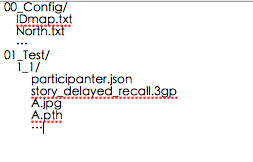
\includegraphics[clip]{OSS_format}
  \caption{阿里云OSS平台上数据存储格式}
\end{figure}

另外,患者的答案也用JSON格式化,也可以参加图3.8。

\subsection{大体框架设计}

系统主要由表达各题目的类和针对题目的界面Activity展示组成。这两个组成部分类似后台和前台,题目的类作为后台储存题目的逻辑部分,并完成一些判分的逻辑;界面Activity可以根据后台的逻辑展现题目,并完成一定的功能,传递数据给后台,让数据能存储到后台部分。这两部分相互独立,又相互依靠。

\subsubsection{题目的类}

\begin{figure}[h]
  \centering
  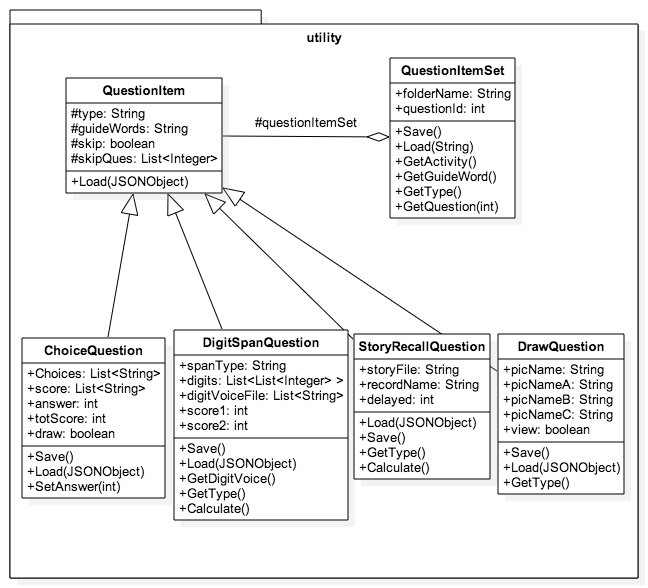
\includegraphics[width=13cm]{question-uml}
  \caption{题目类的UML图说明(部分)}
\end{figure}

所有的题目都基于一个叫做QuestionItem的基类(可见图3.10UML图),而继承的类可以根据其子成员type判断类型,这样即可以保证不同类型的题目可以按照自己的特征存储,保证了题目的完整性也保证了不会有信息冗余性;也可以保证前后台相互独立,可以分开开发。每个题目的类与对应题目格式化得到的JSON相对应,如ChoiceQuestion对应的选择题,成员变量Choices表示各选项的题目,成员变量score表示各选项的分数,成员变量answer表示患者选择的答案,成员变量totScore表示患者最终的得分,成员变量draw表示该选择题是否为图形选择题;而它的成员函数Save()为界面Activity提供了存储答案的接口,成员函数Load()可以从一个JSON中读入题目的各特征,成员函数SetAnswer()给界面Activity提供了传递患者答案的接口。

注:题目的类的集合QuestionItemSet作为整个APP的全局变量(Application)存在,方便整个APP运行过程中题目的读取和答案的保存。QuestionItemSet会在初始界面StartActivity里进行初始化。

\subsubsection{界面Activity}

\begin{figure}[h]
  \centering
  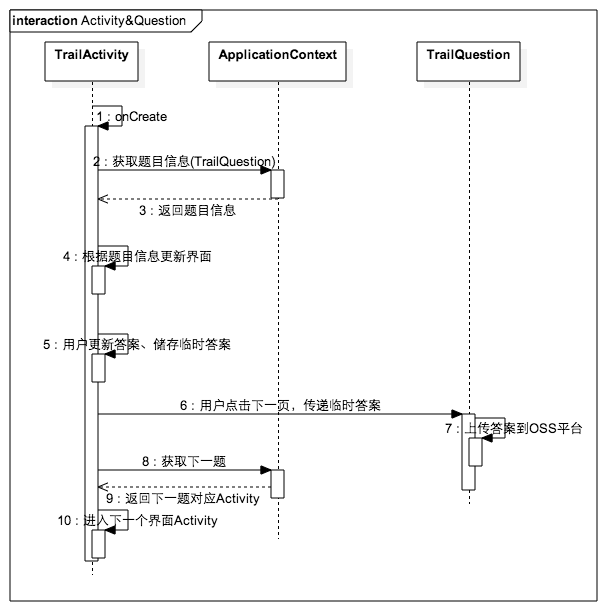
\includegraphics[width=13cm]{interaction}
  \caption{交互设计演示图(以单词配对题为例)}
\end{figure}

对应每个题目有一个对应的Activity来展现其题目,并实现收集数据、传递数据的功能。在初始化界面时,每个Activity从全局变量获取到需要展示的题目,根据其题目的类型和题目中的特征(如guideWords、选择题的选项)设置界面上的一些参数或一些需要播放的媒体文件(如录音题的一些音频)。然后根据用户对界面的操作(如对按钮的点击、修改文字等等)传递数据给后台,或是计算分数。当用户点击“下一页”时,根据后台给出的下一题类型,选出对应的Activity进行展示。

这样将题目的类、界面Activity分开,但相对应的设计,不仅使得开发过程中更为方便、不受干扰、便于调试,使得每种题目类型只需要实现一次,就可以“一劳永逸”;并且使得如果后续需要增加新的题目类型,也可以很方便的进行扩展性。
